% !TEX TS-program = pdflatex
% !TEX encoding = UTF-8 Unicode

% This is a simple template for a LaTeX document using the "article" class.
% See "book", "report", "letter" for other types of document.

\documentclass[11pt]{article} % use larger type; default would be 10pt

\usepackage[utf8]{inputenc} % set input encoding (not needed with XeLaTeX)
\usepackage{listings}
\usepackage{color}
\usepackage[utf8]{inputenc}

% Default fixed font does not support bold face
\DeclareFixedFont{\ttb}{T1}{txtt}{bx}{n}{12} % for bold
\DeclareFixedFont{\ttm}{T1}{txtt}{m}{n}{12}  % for normal

% Custom colors
\usepackage{color}
\definecolor{deepblue}{rgb}{0,0,0.5}
\definecolor{deepred}{rgb}{0.6,0,0}
\definecolor{deepgreen}{rgb}{0,0.5,0}

\usepackage{listings}

% Python style for highlighting
\newcommand\pythonstyle{\lstset{
language=Python,
basicstyle=\ttm,
otherkeywords={self},             % Add keywords here
keywordstyle=\ttb\color{deepblue},
emph={MyClass,__init__},          % Custom highlighting
emphstyle=\ttb\color{deepred},    % Custom highlighting style
stringstyle=\color{deepgreen},
frame=tb,                         % Any extra options here
showstringspaces=false            % 
}}


% Python environment
\lstnewenvironment{python}[1][]
{
\pythonstyle
\lstset{#1}
}
{}

% Python for external files
\newcommand\pythonexternal[2][]{{
\pythonstyle
\lstinputlisting[#1]{#2}}}

% Python for inline
\newcommand\pythoninline[1]{{\pythonstyle\lstinline!#1!}}


%%% Examples of Article customizations
% These packages are optional, depending whether you want the features they provide.
% See the LaTeX Companion or other references for full information.

%%% PAGE DIMENSIONS
\usepackage{geometry} % to change the page dimensions
\geometry{letterpaper} % or letterpaper (US) or a5paper or....
% \geometry{margin=2in} % for example, change the margins to 2 inches all round
% \geometry{landscape} % set up the page for landscape
%   read geometry.pdf for detailed page layout information

\usepackage{graphicx} % support the \includegraphics command and options
\usepackage{hyperref}
% \usepackage[parfill]{parskip} % Activate to begin paragraphs with an empty line rather than an indent

%%% PACKAGES
\usepackage{booktabs} % for much better looking tables
\usepackage{array} % for better arrays (eg matrices) in maths
\usepackage{paralist} % very flexible & customisable lists (eg. enumerate/itemize, etc.)
\usepackage{verbatim} % adds environment for commenting out blocks of text & for better verbatim
\usepackage{subfig} % make it possible to include more than one captioned figure/table in a single float
% These packages are all incorporated in the memoir class to one degree or another...

%%% HEADERS & FOOTERS
\usepackage{fancyhdr} % This should be set AFTER setting up the page geometry
\pagestyle{fancy} % options: empty , plain , fancy
\renewcommand{\headrulewidth}{0pt} % customise the layout...
\lhead{}\chead{Serena Booth $\bullet$ Computer Graphics }\rhead{}
\lfoot{}\cfoot{\thepage}\rfoot{}

%%% SECTION TITLE APPEARANCE
\usepackage{sectsty}
\allsectionsfont{\sffamily\mdseries\upshape} % (See the fntguide.pdf for font help)
% (This matches ConTeXt defaults)

%%% ToC (table of contents) APPEARANCE
\usepackage[nottoc,notlof,notlot]{tocbibind} % Put the bibliography in the ToC
\usepackage[titles,subfigure]{tocloft} % Alter the style of the Table of Contents
\renewcommand{\cftsecfont}{\rmfamily\mdseries\upshape}
\renewcommand{\cftsecpagefont}{\rmfamily\mdseries\upshape} % No bold!
\usepackage{setspace}

%%% END Article customizations

%%% The "real" document content comes below...

\title{Generating Trees From L-Systems}
\author{CS175: Computer Graphics \\ Serena Booth}
%\date{} % Activate to display a given date or no date (if empty),
         % otherwise the current date is printed 


\begin{document}
\maketitle

%{
%\centering
%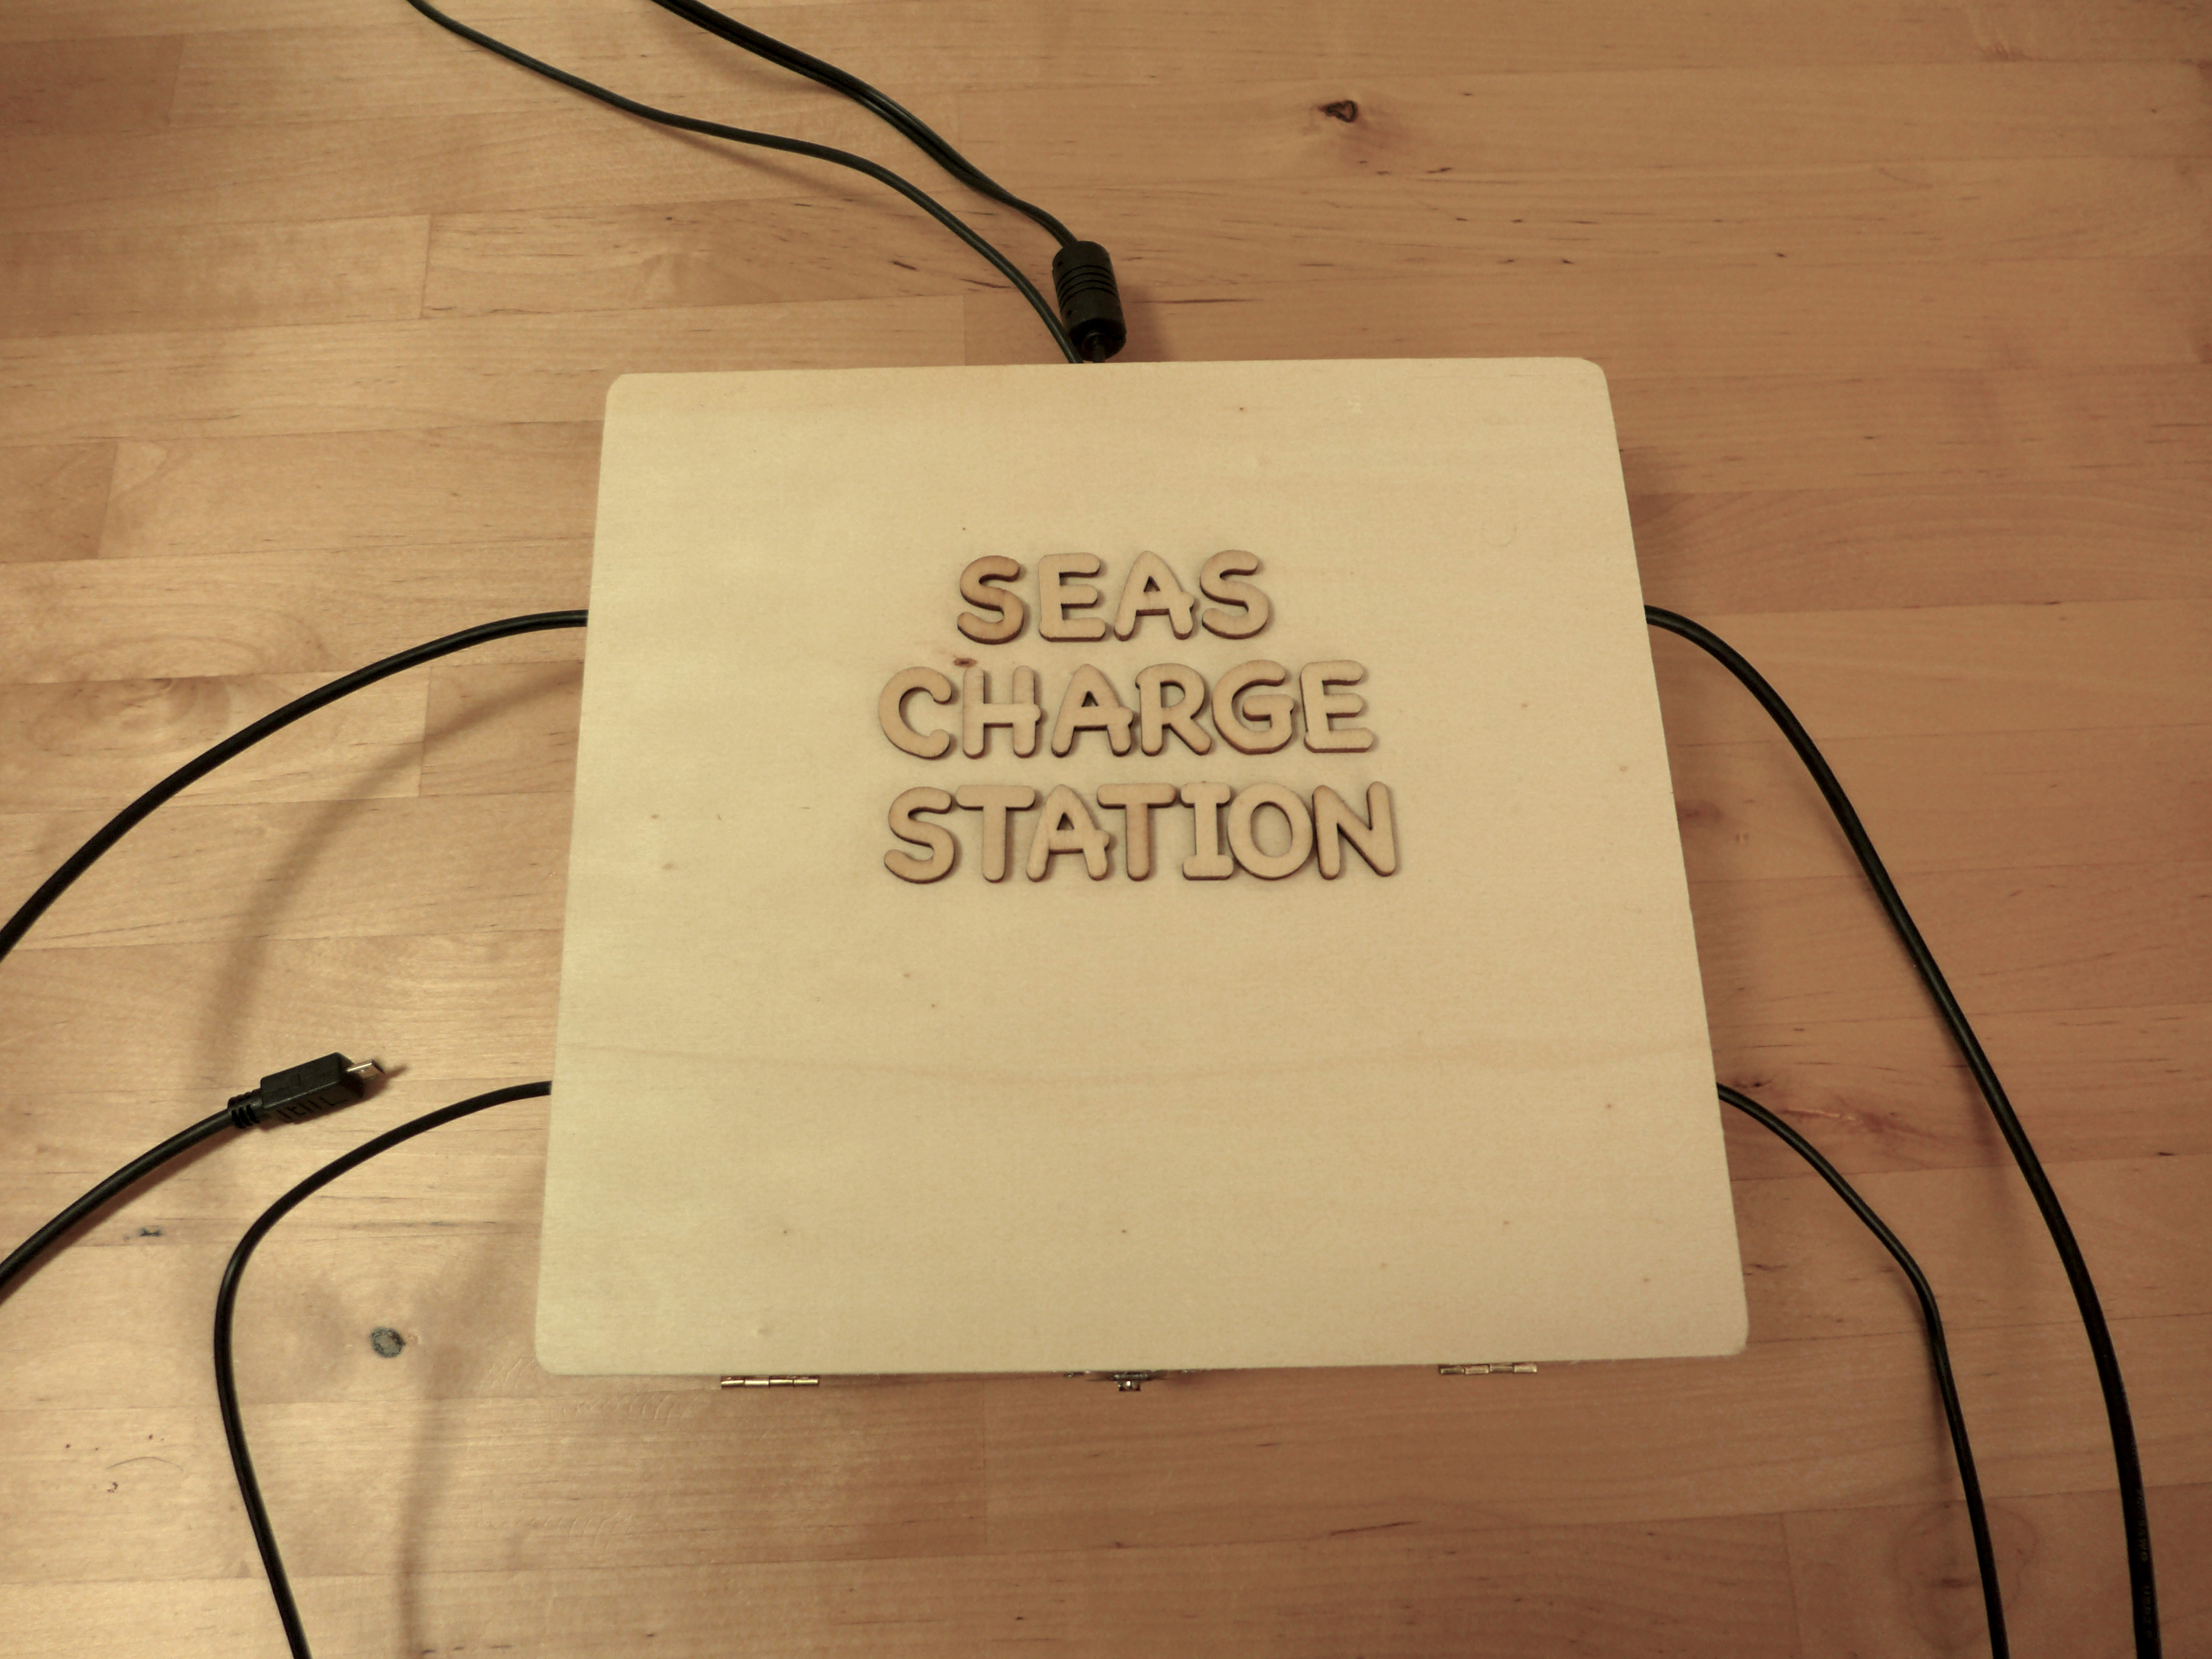
\includegraphics[width=\textwidth]{photo}
%}

\section{Intro} 

I created a tree-generating system. This system uses Lindenmayer, or L-systems, in which a formal grammar describes a tree. The grammar consists of an axiom and a set of rules; the axiom describes the smallest possible tree for a given grammar, and the rules are then applied in order to substitute characters from the axiom to generate a string. My grammars are interpreted stochastically. I parse such a generated string into a scenegraph SgRbtNode. When the tree branches, I add a transform node, and when the tree continues along a branch, I add a shape node representing the branch.  

\section{Hot Keys} 

On running my system -- a make file is provided -- a tree is generated. In order to better interact with the system, I provide hot keys. These processes are detailed here. 

\begin{itemize} 

\item \textbf{ 0: animate the current tree growing! }

How it works: I modified the Drawer class to create a TreeDrawer. This TreeDrawer iteratively draws the tree to a larger depth, starting from a depth of 2 and ending at the depth of the tree as represented in the scenegraph. 

\item  \textbf{1: increase the recursion of the L-System. }

How it works: I wrote an L-System parser which takes an axiom and a set of rules and iteratively applies the rules to the axiom or the generated string. On startup, my system applies the rule set to the axiom 6 times. I keep track of a global variable indicating the depth to which I wish to generate. On pressing `1', this variable is incremented, and the tree is removed from the scenegraph, regenerated, and re-added to the scenegraph. 

\item\textbf{ 2: decrease the recursion of the L-System. }

How it works: see `1'. In this instance, the global variable is decremented, but the approach is the same. 

\item \textbf{3: grow a different L-System. }

How it works: I provide 6 L-System grammars to demonstrate the trees these systems can produce. On pressing `3', I read the next L-System, apply its rules to its axiom some number of times, remove the existing tree from the scenegraph, grow the new tree, and re-add this new tree to the scenegraph. 

\item \textbf{4: increase tree branch thickness. }

How it works: tree branches are represented by cylinder geometry. I initialize such a cylinder to have a height of 1 unit and a radius of 1 unit. When I add this cylinder to the tree, I stretch it in x, y, and z dimensions. Thus I am able to track an overall branch thickness global variable, and increase this variable in order to increase branch thickness. This thickness variable is multiplied in to the stretch factor. As above, I then remove the existing tree from the scenegraph, generate a new tree, and add this new tree into the scenegraph. 

\item \textbf{ 5: decrease tree branch thickness. }

How it works: see `4'. In this instance, the global variable is decremented. 

\item \textbf{ 6: increase branch length. } 

How it works: see `4'. In this instance, I stretch the cylinder's height when before I was stretching its radius. 

\item \textbf{ 7: decrease branch length. } 

How it works: see `4'. In this instance, I shrink the cylinder's height. 

\item \textbf{8: turn off leaves. }

How it works: a global variable toggles the presence of leaves on the tree on and off. On pressing this hot key, the existing tree is removed from the scenegraph, a new tree without (or with, respectively) leaves is generated, and this resultant tree is re-added to the scenegraph. 

\item \textbf{9: simulate leaves moving. }

How it works: in order to achieve a partial wind effect, I allow the user to press the hot key `9'. This removes the existing tree from the scenegraph, generates a new tree, and adds this tree to the scenegraph. This new tree differs in one major way: it includes transform nodes between all the branches and all the leaves.  From this point, I call the function leafAnimateTimerCallback, which adjusts the rotation of the transform nodes. All of the leaves move in parallel, and the effect is designed to be reminiscent of leaves blowing in the wind. This simulation ends when the user presses `9' again. 

\end{itemize} 

\section{L-Systems, Interpretation, and Results} 

\subsection{Interpretation} 

I use a uniform set of variables in my L-Systems. The character `X' is used as a placeholder for generating future iterations. The character `F' means move forward in this direction - e.g. place a cylinder at this location. The character `-' means move -30$^\circ$, plus or minus $0$ to $5^\circ$ randomly in one of the X, Y, or Z dimensions as viewed through the cylinder's frame of reference; the character `+' means the same, but 30$^\circ$, plus or minus $0$ to $5^\circ$, instead. The character `[' indicates the start of a branch; the character `]' indicates the end of a branch. On seeing one of these start branching characters, I push the tree's current state onto a stack, and return to that state on seeing the branch's end.

\subsection{Trees generated from L-Systems} 

{
\centering

\textbf{l0.txt} 

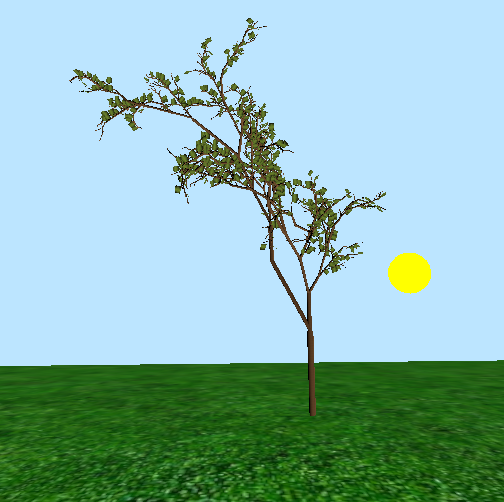
\includegraphics[width=0.5\textwidth]{001}

Axiom: X

X $\rightarrow$ -F[-X+X]+F[-X+X]

F $\rightarrow$ FF

}
\newpage{}
{
\centering

\textbf{l1.txt} 

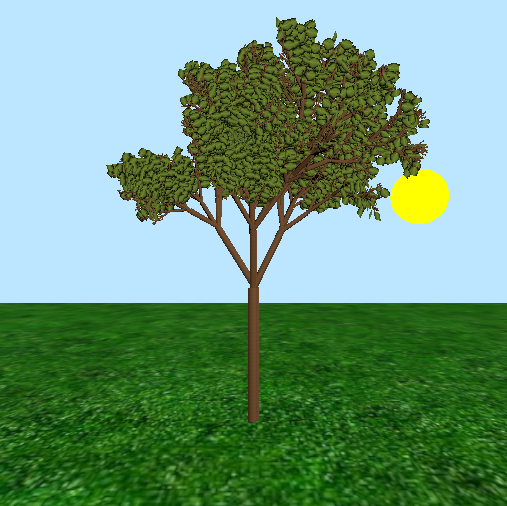
\includegraphics[width=0.5\textwidth]{002}

Axiom: X

X $\rightarrow$ F[-X+X][+X-X][-X+X][+X-X]

F $\rightarrow$ FF

}

{
\centering

\textbf{\\l2.txt} 

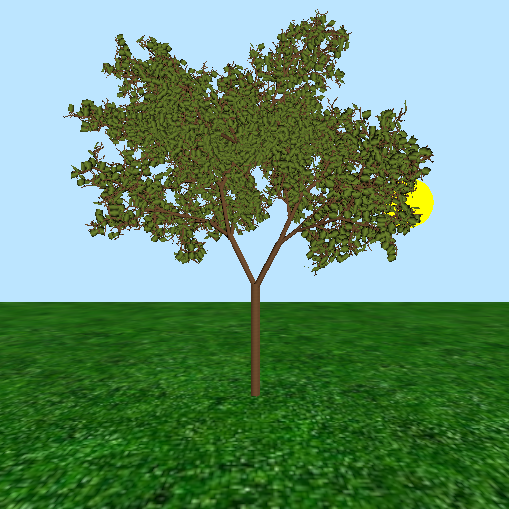
\includegraphics[width=0.5\textwidth]{003}

Axiom: X

X $\rightarrow$ F-[-X-X+X+X]+[+X+X-X-X]

F $\rightarrow$ FF

}
\newpage{}
{
\centering

\textbf{l3.txt} 

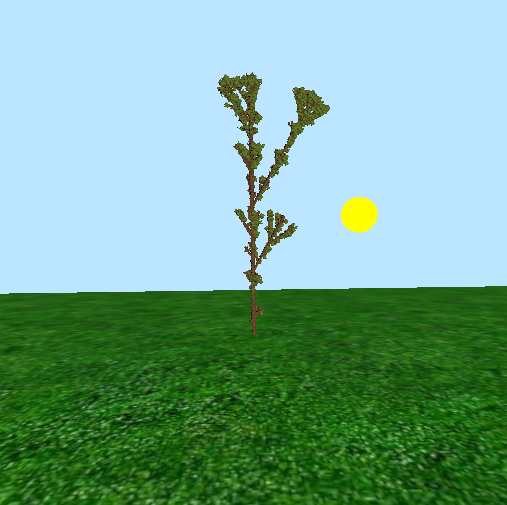
\includegraphics[width=0.5\textwidth]{006}

Axiom: F

F $\rightarrow$ F[+F][-F]F


}
{
\centering

\textbf{\\l4.txt} 

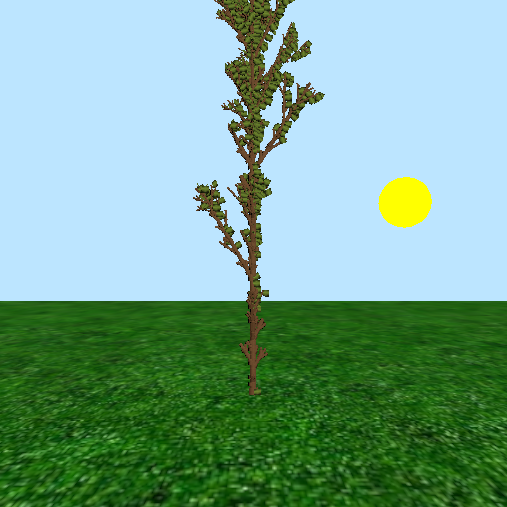
\includegraphics[width=0.5\textwidth]{004}

Axiom: X

X $\rightarrow$ F-[-X+X]+[+X-X]

F $\rightarrow$ FF


}
\newpage{}
{
\centering

\textbf{l5.txt} 

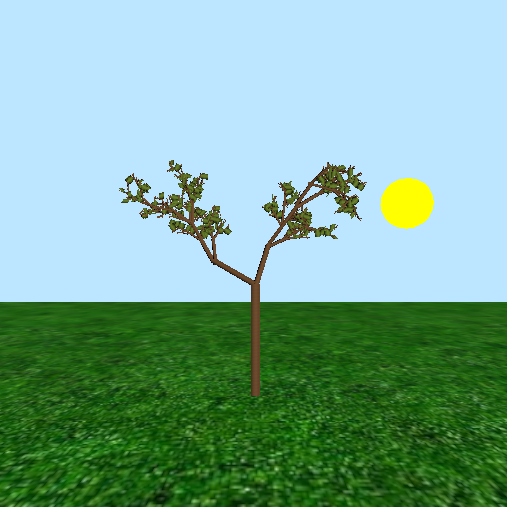
\includegraphics[width=0.5\textwidth]{005}

Axiom: F

F $\rightarrow$ FF[+F][-F][F]


}

\section{Difficulties \& Hacks} 

My main difficulties in this project have been issues of complexity. A tree generated by one of these grammars (e.g. L2.txt), for 6 iterations will generate a string of over 800,000 characters. Interpreting this string gives a tree with over 400,000 transform nodes, and more than 100,000 leaves. Because of this complexity and the depth of the generated scenegraph, rendering such a tree takes a significant amount of time on my machine. In response to this complexity I have considered simple optimizations. For example, the tree is represented by cylinders, each of which contain 12 vertices. I could simplify this tree somewhat by substituting simpler geometry, such as a rectangle, when the branch width is sufficiently small. As is perhaps expected, this optimization did not dramatically increase runtime, so I disabled it in favor of a more uniform tree appearance. 
\\ \\
\noindent I likewise had a difficulty in rendering the leaves on the trees. The leaves consist of very flat rectangles with a textured geometry on top. The texture is represented by a .ppm file. This file contains a leaf against a black background, so in the fshader, I check the color of the fragment under consideration. If the texture at this location is black, I want this fragment to have an alpha value of 0. If the texture at this location is part of the leaf, I want to render that leaf. However, I do so in no particular order, and am not reasonably able to order the leaves from front-to-back by distance due to the scale of the operation. Without this, however, the leaves look broken when rendered. I thus opt to disable the GL\_DEPTH\_TEST when rendering the leaves. 

\section{Personal Take Aways} 
I enjoyed learning about how formal grammars can represent natural phenomenon, and found the results extremely compelling, even from a simple system. 
\\ \\ 
\noindent I found the representation of the tree -- both in using the scenegraph for this data structure and in creating cylinders, leaves, textures, and relationships between those components -- challenging. I spent a while considering different cylinder representations -- from a mesh, from geometry, using GLUT's inbuilt cylinder creation tool -- and found that reflecting on this gave me more perspective on graphics geometry. I ultimately chose to create the cylinder directly from geometry, with the assistance of a resource credited below. 
\\ \\ 
\noindent Unexpectedly, I also found this project taught me a great deal about object oriented programming and design. I haven't done a lot of OO coding at Harvard, and interacting with this system, and its many moving parts -- from the Drawer class to my own LSystem class -- was enlightening. 
\\ \\ 
\noindent Inspired by this project, I also made a trek out to the Museum of Science Pixar exhibit :). 

\section{Resources} 

\begin{itemize} 

\item Prusinkiwicz, P.; Lindenmayer, A. \emph{The Algorithmic Beauty of Plants.} 2004. 

This book provided inspiration, an understanding of L-systems, and some simple L-system grammars which I used and modified in my implementation of tree growing. 

\item \url{https://en.wikipedia.org/wiki/L-system} 

A good overview of L-systems. L0.txt is a modified version of Example 7 from this resource.

\item  Cylinders, Spheres, and Boxes with Direct3D11 and SlimDX. \url{http://richardssoftware.net/Home/Post/7} 

This website provided code for drawing a cylinder into a vertex and an index buffer. 
\end{itemize} 






\end{document}
